\section{High Energy Particles}
\label{sec:high_energy_particles}
\begin{enumerate}
    \item Introduction to high energy particles, cosmic rays, and neutrinos. The standard model. 
    \item The acceleration mechanisms of cosmic rays and neutrinos., derive the power of a particle undergoing first order Fermi acceleration.
    \begin{enumerate}
        \item The Hillas criterion
        \item Derive the power of a particle undergoing first order Fermi acceleration.
        \item Timescales for acceleration
    \end{enumerate}
    \item Talk about the nature of Cosmic rays
    \begin{enumerate}
        \item The composition of cosmic rays
        \item Energy loss mechanisms of cosmic rays
        \begin{enumerate}
            \item Photopion production
            \item Synchrotron radiation
            \item GZK cutoff
            \item Pair production
            \item local volume limit due to these losses
        \end{enumerate}
        \item Detection
        \begin{enumerate}
            \item Detectors and retracing
            \item Emissivity of local volume
            \item Spectrum
        \end{enumerate}
    \end{enumerate}
    \item Neutrinoes
    \begin{enumerate}
        \item Production 
        \item Flavour mixing
        \item Energy loss mechanism
        \item Detection
        \begin{enumerate}
            \item detectors and difficultu of detection
            \item retracing
            \item Emissivity of local volume? 
            \item Spectrum 
        \end{enumerate}
    \end{enumerate}

\end{enumerate}

In this section one will define and discuss the nature of high energy particles such as high energy cosmic rays(UHECRS) and neutrinos. 

\subsection{Acceleration of high energy particles}
Acceleration of high energy particles is still a complicated problem in astrophysics and there are still many open questions. The main ways of acceleration are through shocks, magnetic reconnection, and one-shot acceleration, and one will go through to varying degree these methods in this section. 

\subsubsection{The Hillas criterion}


Before one delves into macroscopic acceleration models one can start with a bigger picture. By arguing that the acceleration, whatever it may be, needs to be of a certain strength and that the particle being accelerated needs to stay confined within the accelerating region for long enough one can create an upper band on the maximum energy reach by charged particle.
This simple but powerful criterion is called the Hillas criterion introduced in \cite{Hillas_1984}, and is a way of estimating the maximum energy a particle can reach in a given source for a given uniform magnetic field.% (ref hillas)

For relativistic particles with charge $Z$ and energy $\epsilon$ in a magnetic field of strength $B$ one can define the Larmor radius


\begin{equation}
    R_L = \frac{\epsilon}{ZB}
\end{equation}

By arguing that the confinement of a particle to an accelerating region is the same as setting the Larmor radius equal to the size of the source, one can 
easily derive the maximum achievable energy for a particle as follows;% (ref M. Bustamante. https://cds.cern.ch/record/1249755/files/p533.pdf)

\begin{equation}
    \epsilon_{max} = ZBR
\end{equation}

Via this method, one can estimate the potential candidates that can produce the observed high-energy particles. 
The criterion works as an upper boundary of acceleration sources since it does not account for energy loss in the acceleration process or any type of interaction that one could expect to be in turbulent environments.
In figure \ref{fig:hillas_c} one can see the different candidates for the acceleration of two different ions, protons, and iron. One of the candidates is the AGN, which is the focus of this paper.

\begin{figure}
    \centering
    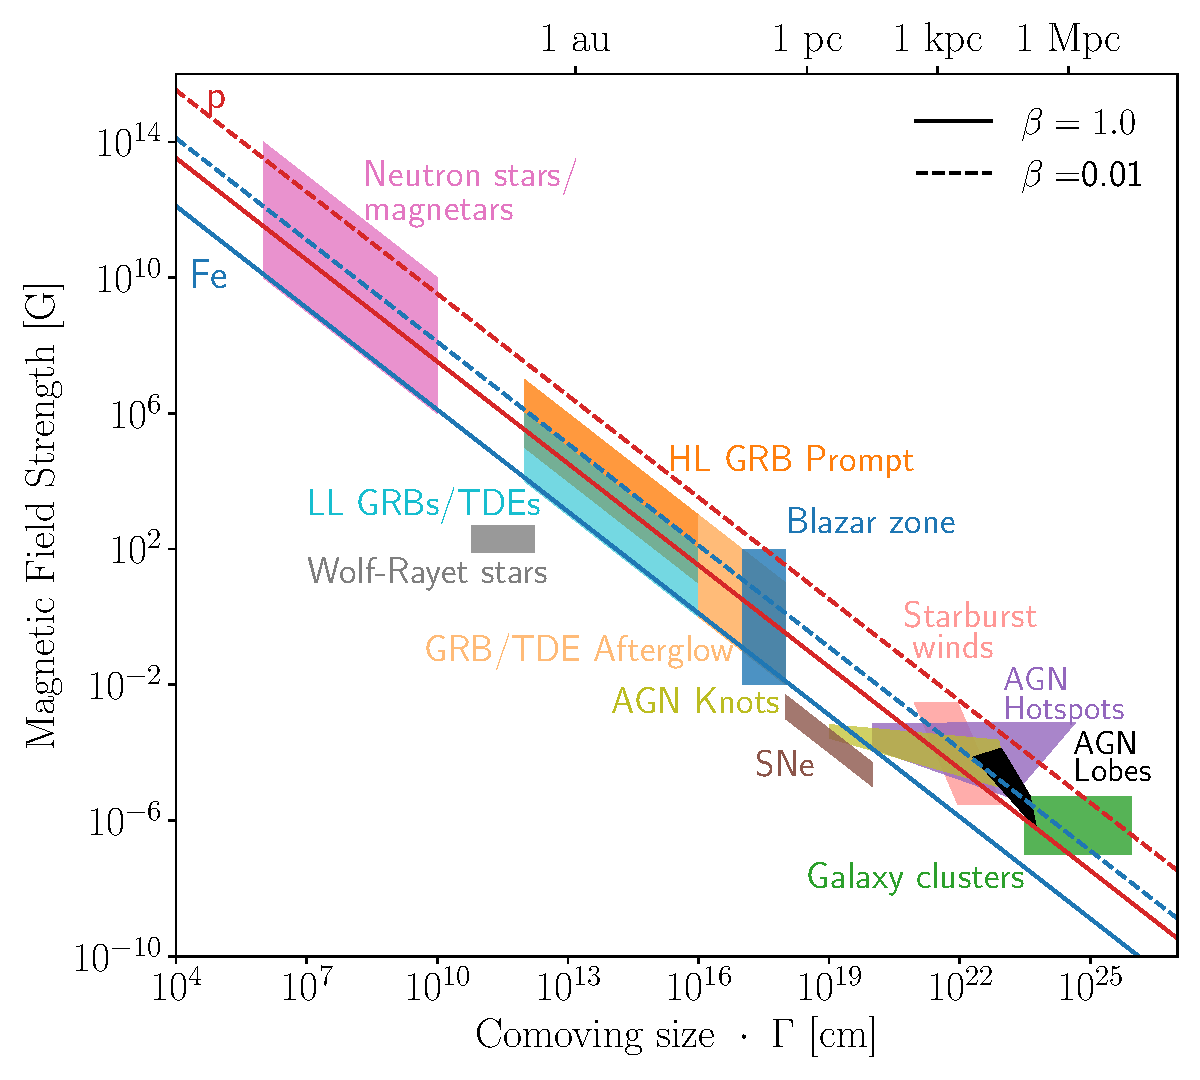
\includegraphics[width = 0.5\textwidth]{C:/Users/henri/OneDrive/Documents/NTNU/Semester 10/Masteroppgave/Plots/hillas.pdf}
    \caption{Hillas criterion for proton (blue line) and iron (red line) accelerated up to $10^{20}eV$ and $10^{21}eV$ respectively}
    \label{fig:hillas_c}
\end{figure}


\subsubsection{Macroscopic Acceleration mechanisms}
In order to accelerate particles to high energies, one needs to have a mechanism that can transfer energy to the particles. This usually happens through electromagnetic fields, and there are several ways this is thought to happen.

\textbf{One-shot acceleration}:
The simplest yet still a powerful way of accelerating particles is through what is called one-shot acceleration. In the presence of an ordered electricmagnetic fields, one can continuously accelerate charged particles which will follow the field lines. This can be induced from a rotating magnetic field or a straight electric field, all which create and electromagnetic force on a hypothetical charged particle. 
This could be the feature of some astrophysical objects such as neutron stars and black holes, usually in a quite close proximity to the object in question.% (ref cern paper)


\textbf{Second order Fermi acceleration/Diffusive acceleration}
In regions where one has high variability in the magnetic field strength, one can accelerate particles via scattering. The idea is that charged particles scatter on what can be seen as magnetic clouds and gain energy in the process due to the speed of the clouds. This mechanism is dubbed second order fermi acceleration due to the average energy gain of a particle being proportional to $(\frac{v}{c})^2$. Here $v$ is the speed of the cloud and $c$ is the speed of the particle. This is a slow process due to the proportionality to $v^2$, but as mentioned in \cite{Dermer_2001} can be a viable way of accelerating particles which already have a high energy. In modern times the magnetic mirrors that particles scatter on are thought to be plasma waves. The idea is that particles occupy a background magnetic field $B_0$ with a superimposed fluctuating electromagnetic field which arrise due to cold-plasma waves. The full formalism is described in \cite{BHradiation} at page 361. In trying to shorten the explination on only focuses on the resulting energy gain. The mean rate of change of the momentum of a particle is given as

\begin{equation}
    \left<\frac{dp}{dt}\right> = \frac{1}{p^2}\frac{\partial}{\partial p}\left[p^2D(p)\right] 
\end{equation}

where the real challenge lies in determining the diffusion coefficent $D(p)$ which is a function of the particle momentum and pitch angle. One will follow the approach found in \cite{O_Sullivan_2009} in which one only considers alfvén waves which take a one-dimensional power spectrum $W(k) \propto k^{-q}$, where $q$ is the spectral index and the total internal energy of the waves is given as $\frac{\delta B^2 }{8\pi}= \int_{k_{min}}^{k_{max}} W(k)dk$.   

As given in \cite{O_Sullivan_2009} the diffusion coefficient with current wave spectrum can be given as

\begin{equation}
    D(p) = \beta_a^2 \frac{\delta B^2}{B_0^2}\left(\frac{r_g}{\lambda_{max}}\right)^{q-1} \frac{p^2c^2}{r_g c}
\end{equation}

where $\beta_a = \frac{B}{\sqrt{4 \pi n_p m_p}c}$ is the alfvén speed, $r_g = \frac{pc}{ZeB}$ is the gyroradius of the particle, and $\lambda_{max}$ is the maximum wavelength of the waves, which will be specified when necessary, but if one is following \cite{O_Sullivan_2009} takes the value of $0.1 R$, i.e. a magnitude lower than the radius of the emitting region.

Form here one can estimate the acceleration timescale of a particle in a given region. The timescale is given as

\begin{equation}
    t_{acc} = \frac{p^2}{D(p)}
\end{equation}


\textbf{First order Fermi acceleration}
In regions where one has strong shock fronts, one can accelerate particles to high energies. These environments can be found several places where the interstellar medium is interacting with a powerful source of energy. One of the most famous examples of this is the supernova remnant where one sees a powerful shock front as a result of a supernova explosion.  
The first-order Fermi acceleration happens when particles traverse these strong shock fronts, and when a particle moves through the shock it gains energy proportional to $\frac{v}{c}$. In addition to this, there is a probability that the particle will stay in the accelerating region and 
experience several accelerations. 

In \cite{Dermer_2001} they can derive the relative power of a particle undergoing first-order Fermi acceleration in a relativistic shock, and it is given as 



\begin{equation}
    \dot p = \frac{2p}{t_u} = \frac{2cqB\Gamma}{mc^2 }
\end{equation}


where $t_u$ is the time in the upstream frame, $p$ is the momentum of the particle, $c$ is the speed of light, $q$ is the charge of the particle, $B$ is the magnetic field strength, $\Gamma$ is the Lorentz factor of the shock, and $m$ is the mass of the particle.

\textbf{KI instabilities in jets}
Another method of acceleration which really is diffusive one shot acceleration related to AGN jets is acceleration via the kink instability in jets. The idea of kink instability leading to acceleration is found in \cite{Alves_2018}. Kink instability is a hydrodynamic instability that arises in jets when the magnetic field is not aligned with the jet. If a perturbation is introduced to the jet, the resulting force on the jet structure will magnify the perturbation. This will lead the jet to a much more complicated structure, and twist the magnetic field lines. See figure \ref{fig:kink_instability} for an illustration. The paper argues that a highly tangled magnetic field and a large scale inductive electric field which is found throughout the kink-unstable region will lead to rapid energization of particles. 

\begin{figure}
    \centering
    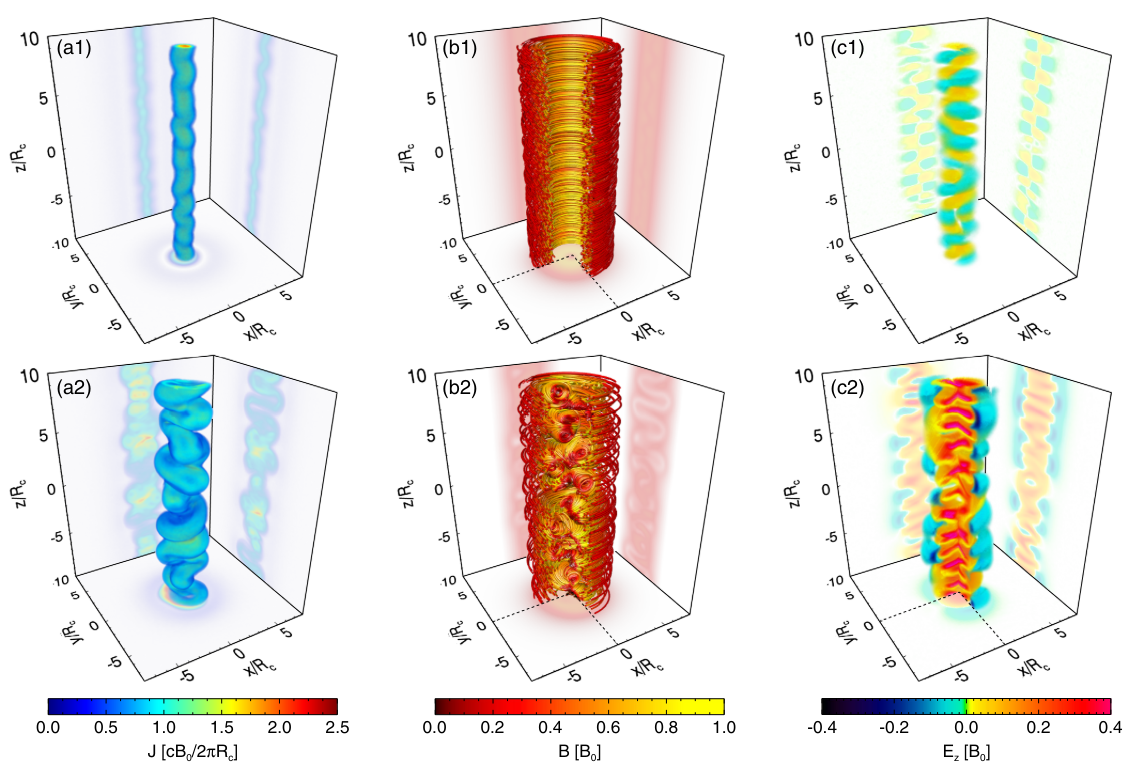
\includegraphics[width = 0.8\textwidth]{C:/Users/henri/OneDrive/Documents/NTNU/Semester 10/Masteroppgave/Plots/KI_instability.png}
    \caption{Simulations from \cite{Alves_2018} showing the evolution of kink instability in a jet. The upper panels shows the before the KI instability has been amplified, and the lower panel shows the jet after the instability has been amplified. From left to right the panels show, Current density, magnetic field lines, and axial electric field. }
    \label{fig:kink_instability}
\end{figure}

\subsection{UHECRs}

UHECRs are charged particles that are bombarding the Earth with energy exceeding 1 exaelectronvolt ($10^{18}$ eV) according to \cite{Alves_Batista_2019}. The origin of 
these particles is still a mystery but due to their high energies, they are thought to be extragalactic in origin.
The composition of UHECRs ranges from protons to heavier nuclei such as helium or iron, and when these particles interact with the atmosphere they produce a shower of secondary particles.
The air showers could also give extra information such as direction, but due to the nature of UHECRs, the location of their source is
difficult to pinpoint. This is because UHECRs are charged particles and therefore are deflected by the magnetic fields they encounter.

\subsubsection{Production and Energy loss}
The requirements to produce a UHECR are a charged particle and a powerful accelerator. But in order to
model them sufficiently one needs to take into account their journey to the Earth. Both during the acceleration and during the journey to Earth, the UHECRs will lose energy. 
The important parameters for this energy loss are its composition and its environment. In addition, as mentioned before, the interstellar magnetic field will also deflect the particles and therefore the direction of the particle will be changed. 
These effects are important parameters since they limit the 
distance a particle can travel before it loses too much energy, and therefore limits the local volume in which high energy cosmic rays can be produced. 
Here I will briefly discuss the different energy loss mechanisms.
